\chapter{Overview and outlook}
\label{sec:overview}


\section{Literature}

Ferromagnetic HEA CoFeMnNiX, X = Al, Cr, Ga, Sn	\cite{ZUO201710}. Mn antiferromagnetism dampend in favour of ferromagnetic phase. Cr pushed the material to a paramagnetic phase. \\

A high entropy silicide  of TM elements: (MoNbTaW)Si2 \cite{GILD2019337}, main result: First real material of this type. And evidence for high-entropy alloy in a non-cubic unit cell (Hexagonal P6222). Low thermal conductivity compared to comperative materials in same crystal stucture NbSi2, TaSi2.  \\

Magnetic properties of eqvimolar CrMnFeCoNi HEA \cite{PhysRevB.96.014437}. Local magnetic moment are Cr align antiferromagnetic. Fe and Mn big and their interaction with the magnetic surroundings are responsible for the magnetic properties of the alloy. Done with DFT and experimental methods. \\

A large-scale project for investigating thermoelectric properties of silicides \cite{doi:10.1063/5.0008198} with DFT. \\

Study showing the promise of beta fesi2 as a thermoelectric and options to increase zT \cite{doi:10.1021/acsami.0c00321} \\

\textbf{Master to Mari:} High-entropy silicides, Cu did not mix well, but found 3 phases with Si Co Cr Fe Ni. First phase: Hexagonal crystal structure, far from eqvimolar with very low Ni and most Cr, ie same as the one permutation I made. But she also found 2 other phases high in Ni in orthorombic stucture. Si occupiyning Si sites in the initial structure. Thermoelectric outcome: Similat electrical resistivity to other known HEAs, but Seebeck coeff was too high for thermoelectric application. \\

LDOS/PDOS bulk beta fesi2 \cite{doi:10.1063/1.346415} that show similar properties to us. \\

A known problem of random alloys is the presence of defect states in the otherwise band gap \cite{PhysRevLett.104.236403}.  \\

Specifics on the Local DOS of various TM silicides \cite{lange1997electronic}, very good agreement with our results. Mention this! \\

\section{General thoughts}

Mention later that the magnetic moment vary between SQSs more in other cases, and not in the eqvimolar, why is this? 

XC results: PBE poor in 3d elements, Ni particularly. But PBE does not overestimate the band gap so if we find a gap with PBE the real material very likely have a band gap and a larger one at that. Reversly the SCAN functional have shown limitations to magnetic compounds, but have shown a good promise of modeling diversly bonded structures as one with both metalic and covalent bonds? And have does improve theoretically on GGA. Next was the hybrid functional that have no known limitations to either band gap calculations or our particular system. The sole drawback is the cost, in figure .. bellow we show the respective computational time in terms of CPU-hours between the 3 different functionals of SQS D. Additionaly, the low number of k-points is a concerning factor and the exagerated band gap of the bulk compound. Nevertheless we find generally good agreement between PBE and HSE06 in which both predict semiconductors with severe polarization in the spin up channel, this is more evident in the HSE06 calculations. \\

Calculate VEC and include in the report. \\

Mention that the first we only tested colinear spin polarization and non-spin polarized calculations for simplicity, thus many many possible magnetic configurations have been neglected. Furthermore all calculations was performed at 0 K, so the magnetic alignment is not necessary representative of the material at different temperatures. And a specific study devoted solely to the magnetic properties of the material is requiered for this. However, as is apperant from the spin polarization of the band gap we do note at least a magnetic character in the alloy, contrary to the bulk FeSi2 material whom we found to be nonmagnetic. \\

Cr and Mn are found to be anti-ferromagnetic elements. In the studies above we see some examples of these in alloys. Also, from section .. we know that SQS struggle with magnetic materials. \\

Mention that there are no band gap to compare to, plus we have already covered a great deal of the computational factors of the gap. Could mention that the local and projected density of states correspond well with transition metal silicide studies. So we will in this section relate other properties of the high-entropy silicide and some additional factors of this study. \\

Mention the impact of only doing 0 K calculations in terms of the band gap and electrical properties, magnetism and stability. And relate this to the focus of this project of only locating potentially promising materials and provide some initial properties. But the intention is that this is a starting point for further investigation at finite temperatures and such necassary for practical application of the material. \\

Mention that FeSi2 structures in this project does not fit in the frame of a HEA material/study, but it is a new class of material, and the one study does help. Mention in begining of results that are initial attempt was a (CrFeCoNi)2Si HEA based on the Fe2Si crystal structure but found no sucsess, therefore we did as we did. \\

Mention in introduction that a key property of a thermoelectric is a narrow band gap, therfore by high-entropy stabilization and reduction of the phonon scattering it's hope for high zT values. \\


\paragraph{The SQS size}

Lastly a precise determination of the exact value of the band gap would requiere much more effort. Recalling the concerns of the special quasi-random structures, we know that one problem is the large possible number of configurations. Here we select only a span of 5 and we find that the band gap varies greatly between all 5 but show the same characther. Thus we should have performed a larger search over more configurations. Additionly also the SQS size is relevant, here we have only tested a 48 atom model, but as section .. stated often much larger SQSs are required to reach convergence and accuratly model the disordered structure of HEA. At the same time this is not a true disordered structure, the Si atom contain some order and this is not really a typicial HEA so maybe this is not as important.

In this project we have made calculations of a type of supercell and SQS model. This model consisted of 48 atoms and have a volume of $700 Å^3$ before structural relaxation. This was done for two reasons, firstly it allowed for the use of more complex XC-functionals, and secondly enabled a broad study of distinct permutations and compositions. However, as covered in section 4.2 or something the results of the SQS model is known to show a sensitivity to the size of the model. For this reason we include the results of 96 and 192 atom SQSs of \ch{CrFeMnNiSi2} with volume $1200 Å^3$ and $2400 Å^3$ respectively. Bellow in figure .. we show the increased computational burden in terms of cpu-hours from performing both structural and ionic relaxation as well as a single electronic self-consistent calculation with PBE GGA of the distinct SQSs. 

\begin{figure}[H]
\centering
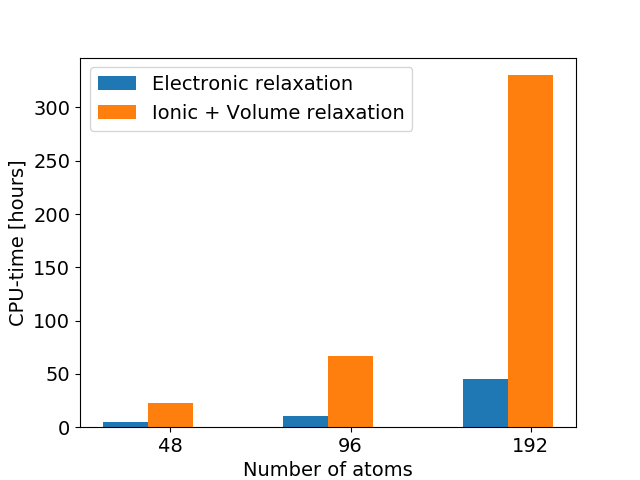
\includegraphics[width=.8\textwidth]{results/SQS_time.png}
\end{figure}

\begin{table}[h!]
%\centering
\hskip-2cm\begin{tabular}{@{}cccccc@{}}
\toprule
       & \multicolumn{2}{c}{Total energy/atom (eV)} & Enthalpy of formation (eV) & \multicolumn{2}{c}{Final magnetic moment ($\mu_B$)} \\ \midrule
48 atoms & - 6.6105 & .. & -11.5000 & 0.0833 & 0.0000    \\
96 atoms & - 6.6092  & 0.0021 & - 22.8752  & 0.0708  & 0.0114     \\
192 atoms & - 6.6123  & 0.0022 & - 46.6654 & 0.0761 & 0.0171     \\ \bottomrule
\end{tabular}
\caption{Mean and stadard deviation of the total energy and magnetic moment per atom, plus enthalpy of formation of the listed mean energies (\ch{FeSi2}).}
\end{table}


\begin{figure}[H]
\begin{subfigure}{\textwidth}
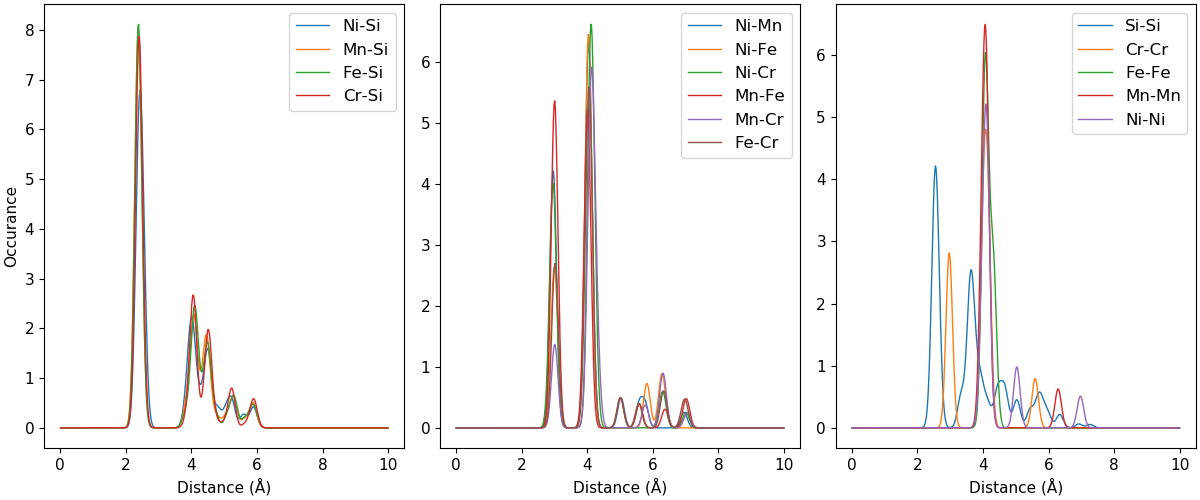
\includegraphics[width=\textwidth]{results/PDF48.png}
\end{subfigure}
\begin{subfigure}{\textwidth}
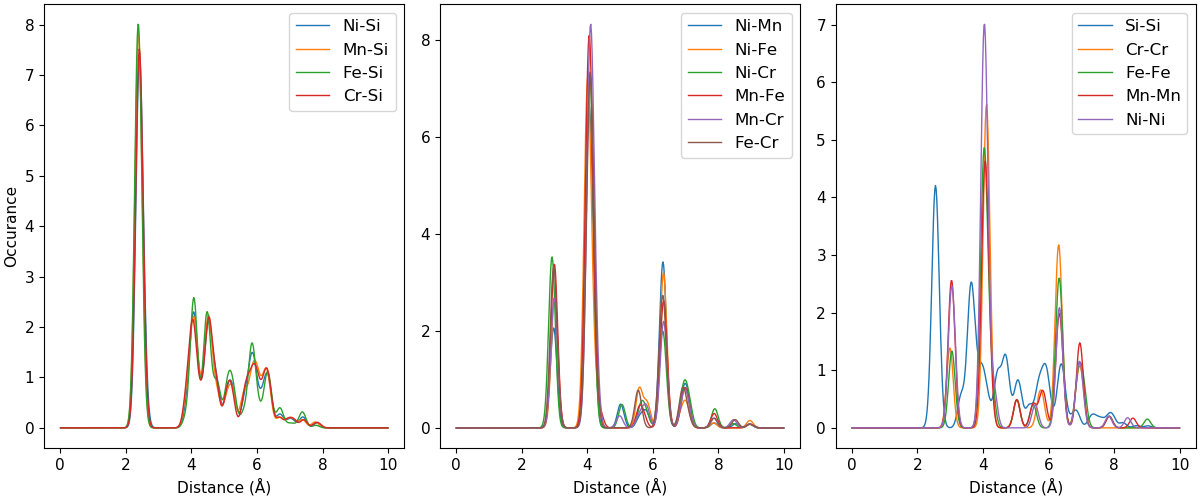
\includegraphics[width=\textwidth]{results/PDF96.png}
\end{subfigure}
\begin{subfigure}{\textwidth}
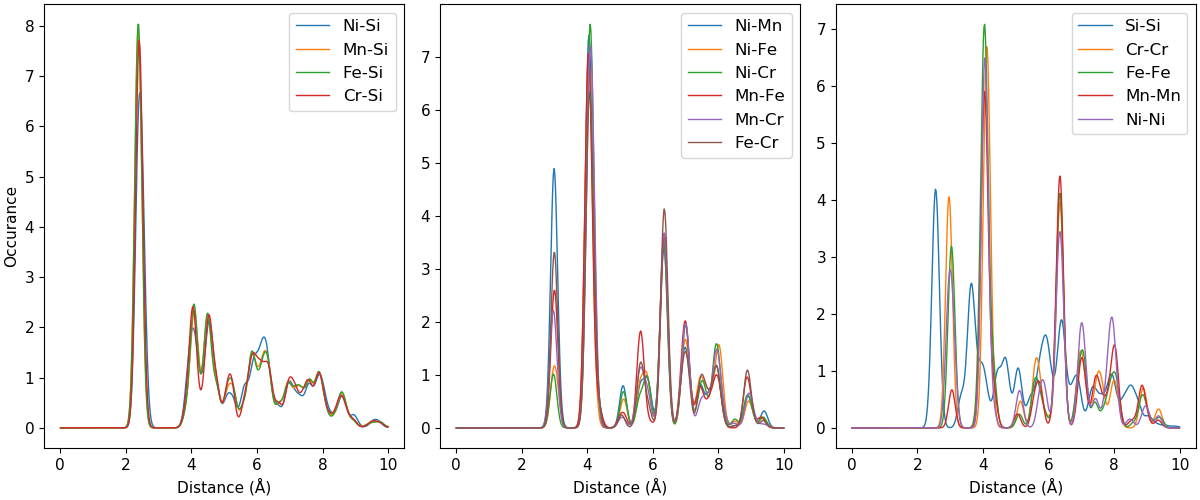
\includegraphics[width=\textwidth]{results/PDF192.png}
\end{subfigure}
\end{figure}


\begin{table}[H]
\centering
\begin{tabular}{@{}ccccc@{}}
\toprule
                                                     &   & Spin up (eV) & Spin down (eV) & Total (eV) \\ \midrule
\multicolumn{1}{c|}{\multirow{5}{*}{\textbf{48 atoms}}}   
												  & A & 0.0815                & 0.0521                  & 0.0281              \\
\multicolumn{1}{c|}{}                                & B & 0.2932                & 0.0523                  & 0.0523              \\
\multicolumn{1}{c|}{}                                & C & 0.2355                & 0.0343                  & 0.0343              \\
\multicolumn{1}{c|}{}                                & \textbf{D} & 0.3386                & 0                       & 0                   \\
\multicolumn{1}{c|}{}                                & E & 0.3078                & 0.0495                  & 0.0495              \\ \midrule
\multicolumn{1}{c|}{\multirow{5}{*}{\textbf{96 atoms}}}   
                                                     & \textbf{A} & 0.1705                & 0.0442                  & 0.0367              \\ 
\multicolumn{1}{c|}{}                                & B & 0.1386                & 0.0270                  & 0.0270                   \\
\multicolumn{1}{c|}{}                                & C & 0.1347                & 0.0363                  & 0.0075                   \\
\multicolumn{1}{c|}{}                                & D & 0.0892                & 0.0398                  & 0.0398                   \\
\multicolumn{1}{c|}{}                                & E & 0.1610                & 0                       & 0                        \\ \midrule
\multicolumn{1}{c|}{\multirow{5}{*}{\textbf{192 atoms}}}
	 									           & A & 0.1197                & 0.0321                  & 0.0321                   \\
\multicolumn{1}{c|}{}                                & B & 0.1444                & 0                       & 0                        \\
\multicolumn{1}{c|}{}                                & C & 0.1867                & 0                       & 0                   \\
\multicolumn{1}{c|}{}                                & D & 0                     & 0                       & 0          \\
\multicolumn{1}{c|}{}                                & \textbf{E} & 0.0131                & 0.0184                       & 0.0131                   \\ \bottomrule
\end{tabular}
\caption{Total and spin dependent band gap of 4 permutations of CFMN (fesi2) with PBE GGA calculation. The structures that are excluded from this list either failed in calculations, or does not show any band gap.<}
\end{table}

\section{Other things}

blablabla, Cr is known to lower the saturation magnetization in HEAs, we observe an opposite effect. SQS struggle with paramagnets, furthermore with specific compoitions, therfore maybe the method is poor suited for our case. Similarly PBE is known to be of limited use in 3d elements, SCAN for magnetic but good for diversly bonded structures. HSE06 is overall the best, same for MBJ, but both proved difficult to implement on large-scale for such complex materials. Bellow is a table illustrating a the computational demand for CrFeMnNiSi2 sqs D between the 3 methods. 

Finally we show a figure of the overview of all results in this project. In it we have also included the results of the CrFeMnSi based alloy built from different initial starting points such as the CrSi2, MnSi175 and Fe2Si that inlcude different metal-Si ratioes and crystal structures, par Fe2Si the materials are known semiconductors with band gaps above 0.5 eV. As the figure show, none of these showed any indication of a band gap, this applies for half-metal gaps as well. As a positve, we observe that the positve FeSi2 results are also the most stable structure of this compostional HEA silicide based on the calculated formation enthalpies.  

 We find that the half-metals and/or semiconductors are somewhat magnetic according to our own calculations. Compared to FeSi2 cmce bulk which is anti-ferromagnetic, we experience that alloying this structure with different 3d elements in a HEA method yields a magnetic moment.  But we should balbla study this at elevated temperatures for a proper description of the magnetic properties of the alloy. This result was mearly included to present an overview over potential properties and applications of this material. However the magnetic charachter is certainly evident from the large spin polarization of the band gap. This makes for many interesting applications, for instance within the spin-tronic sector. The Half-Metal property is in line with relevant studies of similar studies, see .., which point to spin-gapless semiconductors. We can not conclude this result of the alloy becouse we have not considered the various conductivites amongst other relevant properties. But the band gap insinuate that this could be the case. Furthermore from the magnitude of the gap, this alloy could have promise as a thermoelectric material. High-entropy alloys is known to heavily lower the phonon scattering in materials which is a desirable property of TE's for a high figure of merit. However HEAs also show low electrical conductivity as well, this is bad for TE's. However from the band gap size this is worth a focused study on it's application in thermoelectricity. See for example Mari master that found some positive effect of a similar material. \textbf{Anything else?}

\paragraph{Numerical smearing \\}

One final point we would like to cover in the discussion of HSE06 calculations of this system, and generally in this project, is the effect of smearing on the reported band gaps. From the method section, we know that TBC smearing is the preferred choice for accurate density of states and total energy calculations of semiconductors, alike we know that this method is unfitting to calculate the forces in metals. As discussed in the methodology section, hybrid functionals proved difficult to converge for such composistionally complex structures, thus we were forced to initially calculate the charge density from the HSE06 functional with did a self-consistent calculation with gaussian smearing and smearing width of 0.05 eV. Thereafter reuse the calculated charge density for subsequent hybrid calculations with TBC smearing. Using SQS A as an example, from the first run (Gaussian), the band gap is 0.15 eV, (0.78 up and 0.15 down). However the eigenvalues contain defect states and the band gap is not observable from the density of states. Next we can reapply the charge density to perform an additional HSE06 calculation with gaussian smearing, but reducing the smearing width from 0.05 eV to 0.005 eV. Now we find a new gap of 0.1 eV (0.21 up and 0.1 down), with no defects in the eigenstates, and apperant in the density of states. In cases where we find conflicting results between the eigenvalues and density of states we rely on the script bandgap.py provided in the pymatgen package, refer to section .. for a description. With this we only report a band gap for the HSE06 calculation with TBC smearing, note that this method return the same value of the gap as well. As another example lets consider SQS B. In contrast, the nummerical smearing does not appear to impact the band gap of this structure. We find from HSE06 simulations with gaussian smearing of both 0.05 and 0.005 eV smearing width to yield results around 0.28 eV and 0.18 eV in spin up and down. But alike SQS A, the larger smearing width comes with a few defect states in the spin down channel and additionally can not be seen in the density of states. However, particular of this structure is that the bandgap.py script validate the calculated total band gap from the eigenvalues in all three calculations. Aside from this abnormalty, the other SQS similar to A find some similarities between smearings, but only TBC was validated with bandgap.py, furthermore the DOS does not with the same clarity reproduce the calculated band gap from the eigenvalues in calculations done with gaussian smearing compared to TBC. \textbf{figureof the DOS of hybrid/smear/smear5 maybe A?}

We see from the above examples that as most studies and articles state, that TBC smearing is superior in terms of accurate total energy and DOS calculations of semiconductors. Similar to how TBC produce inacurate forces of metals, in several cases in this project we relaxed the structures with gaussian to forces bellow 1E-2, but subsequent calculation with TBC in certain cases resulted in forces above 0.1, without making any geometric alteration to the previously relaxed cell \textbf{(Include examples?)}. On the grounds of these factors we can report good agreement between our own results and the theoretical advice regarding numerical smearing in DFT studies \textbf{Insert refrence vaspwiki}

\textbf{Other shit}

\textbf{EIGENVAL stuff}
To explain the result of SQS D in comparison to the other semiconducting SQSs of the alloy, we look at the calculated eigenvalues for the distinct supercell. Here it's seen that eigenstates transition between full to empty occupancy at energy band 124 in spin down and 129 in spin up, thus a difference of 5 bands between states in the different spins, this is also the case in the other SQSs. In particular of SQS D however is that for a majority of k-points the bands 124 and 125 contain occupancy values other than 1 and 0 for the spin down states. These are either non-physical values above 1 or negative, in other words indicating states are more than filled or less than empty. Or values in-between 1 and 0, meaning partially filled states (defect states). If we were to neglect these defect states and only consider bands where the occupancy is above 0.99 or bellow 0.01, the band gap of structure D remain consistent in spin up, but we now observe a band gap of around 0.05 eV in the spin down channel as well. Again, this would have been extremely insightful to investigate with the help of a band structure diagram. The non-physical values is simply a consequence of using the tetrahedron method with Bloch corrections (ISMEAR-5) as numerical smearing, (\textbf{Insert reference}). Interestingly we only find such values for spin channels also containing defect states. Furthermore the presence of such defect/non-physical states is found as the key divider between structures with and without a band gap also for the coming examples in this project. \\\\


\textbf{Point of k-points and HSE06 results}
One possible reason behind the abnormally large gap can originate from the small number of k-points we had to employ in order for the calculations to converge. Recalling that the gap transition in in the PBE calculation was (0.250,0.000,0.250)-(0.000,0.000,0.000), compared to the hybrid functional we now see that the transition is between k-points (0.500,0.000,0.000) and (0.000,0.000,0.000). Moreover, the point (0.250, 0.000, 0.250) in k-space is not included in the hybrid functional due to the narrow mesh (this we read from the IBZKIT file in VASP). Thus it's a possibility that the large gap is caused by the fact that the minimal gap is not encapsulated by the k-points in the HSE06 calculation. However we also see this trend in the other SQSs, but despite of the different transistion in k-space, these structures find lesser band gaps with the HSE06 functional compared to PBE. Additionally, we find similar results in the bulk $\beta-$\ch{FeSi2} structure. In this calculation we applied the same number of k-points for HSE06 as for PBE and SCAN. Nevertheless we find a much larger band gap of around 1.5 eV with HSE06, as opposed to 0.65 eV with both PBE and SCAN, and as mentioned before the two latter is in much better agreement with experimental results and ab intio work on the band gap of $\beta-$\ch{FeSi2} \textbf{cite materials project, other articles}. Additionally also in this case, the transition vary between functionals. PBE: (0.000,0.000,0.000)-(0.000,0.000,0.250), and HSE06: (0.000,0.000,0.000)-(0.000,0.000,0.500).



\section{\ch{Cr4Fe4Mn4Ni4Si32} in different crystal structures}

In the discussion above we have covered in great detail the possibilites of high-entropy silicides based on the $\beta-$ \ch{FeSi2} unit cell with twice as many silicon atoms to 3d elements. The primary outcome and conclsion of this research was that particularly the combination of Cr, Fe, Mn and Ni resulted in superiour properties in the light of the motivatian behind this project. The next question we wish to answer is if ihe promising results of the CFMN system be reproduced in other symetries. In this section we will implement the CFMN composistion in crystal structures based on hexagonal \ch{CrSi2} ($P6_{42\Bar{2}}$), both tetragonal and orthorombic \ch{Mn16Si28} ($P\Bar{4}c2 and$, $Pcca$), and trigonal \ch{Fe2Si} ($P\Bar{3}m1$) where we test the CFMN system to varying metal and silicon ratioes, and crystal structures. As before, the total energy, enthalpy of formation and magnetic moment per atom can be found bellow in table ..
\begin{table}[h!]
\begin{tabular}{@{}cccccc@{}}
\toprule
            & \multicolumn{2}{c}{Total energy per energy} & Enthalpy of formation & \multicolumn{2}{c}{Mag per atom} \\ \midrule
CrSi2       & -6.4837               & 0.0087              & -8.1205             & 0.0887          & 0.0387         \\
MnSi        & -6.6658               & 0.0071              & -9.1848             & 0.0687          & 0.0398         \\
Fe2Si       & -7.5082               & 0.0107              & -10.2474            & 0.3848          & 0.0588         \\ \bottomrule
\end{tabular}
\end{table}

\textbf{CrSi2 \\}
From our calculations with PBE DFT we find the bulk crsi2 material to be an indirect semiconductor with a band gap of 0.33 eV, slightly bellow the listed value of 0.36 eV in materials project \textbf{cite}, suprinsingly we find a smaller gap of 0.32 eV from the SCAN functional. The compound is also nonmagnetic in agreement with materials project. Fore the bulk material we employed a 9 atom cell, with 6 silicon and 3 cr atoms, from this we generated SQSs of 72 atoms with the same ratio.  \textbf{Include toten per atom for the unit cell? and figure of SQS + unit cell?}. For this given composistion and system we observe very similar results to that of the composistions discussed above, the eigenvalues of several SQSs report a small band gap, but its not apperant from neither the density of states or from the bandgap.py script of pymatgen. Additiontly, we can not repreoduce the gap with the SCAN functional, as was possible for the CFMN (fesi2) system.   

\paragraph{MnSi \\}
In the tetragonal configuration, the bulk material is a nonmagnetic indirect semiconductor with a band gap of 0.76 eV acoording to our PBE calculations,  and 0.78 eV from SCAN. Materials project find a band gap of 0.76 eV, in good agreement with our own PBE results. The unit cell consist of 44 total atoms, 16 manganese and 28 silicon. In the orthoromibic cell, with equal number of elements we find a band gap of 0.76 eV (0.77 ev SCAN) as well. In contrast, the CFMN alloy of both these cells produce metalic compounds. It should be noted that structures B and D in the tetragonal ssystem did not fully relax, same for D in the orthorombic cell, so these results could be inaccurate.   

\paragraph{Fe2Si \\}
In this cell, we drasticly alter the metal-silicon ratio, this is seen both in the band gap and magnetic properties of the material. The magnetic moment of this cell consisting of 4 iron atoms and 2 silicon atoms is 0.67, from the iron atoms. This magnetic charachter can also be observed from the discrepency between the two spin channels. In spin down we find a band gap of 0.21 eV, while there is no gap in spin up. This gap can also be seen in the density of states \textbf{Include figure}. This however is an abnormal result in regard to other experimental work and littereature on the Fe2Si \textbf{cite $https://www.sciencedirect.com/science/article/pii/S0925838816329796?casa_token=g9DRpU9IClcAAAAA:6Gd12A4Kh9J2igUWMVwHN8OSIKzD27VACA052FNsSAWhRY6PELWdVEPbiF8OtQ3eJEAbvQ8X0g$}. Our results are subject to errors, particularly we note that the eigenvalues used to calculate the gap contain nonphysical values in the spin down channel. However, the gap is evident in the density of states thus we include the result in this report, but acknowlendge the uncertainties revolving the value. 

From this unit cell we generate 54 atom SQSs. From table .. we see that the magnetic nature remains, producing the overall highest magnetic moment of all studied supercells, which is not a surprising result considering the 3d metal to silicon ratio. \textbf{More on magnetic and total energy.} The magnetism can also be seen in the difference between the two spin channels, the bands where the occupancy transistion from 1 to 0, ie occupied to not occupied is very different. In the most magnetic supercell D, we saw a distance of 22 bands between the spin down transistion and spin down transistion. Most supercells are metals from our PBE calculations. B and D show a very small gap of around 0.01 eV in one spin channel.  In E we find a very narrow gap semiconductor with a total gap of 0.002 eV. This gap is surrounded by the same uncertainties as discussed previosly.  

\section{Overview}

\begin{figure}[H]
\centering
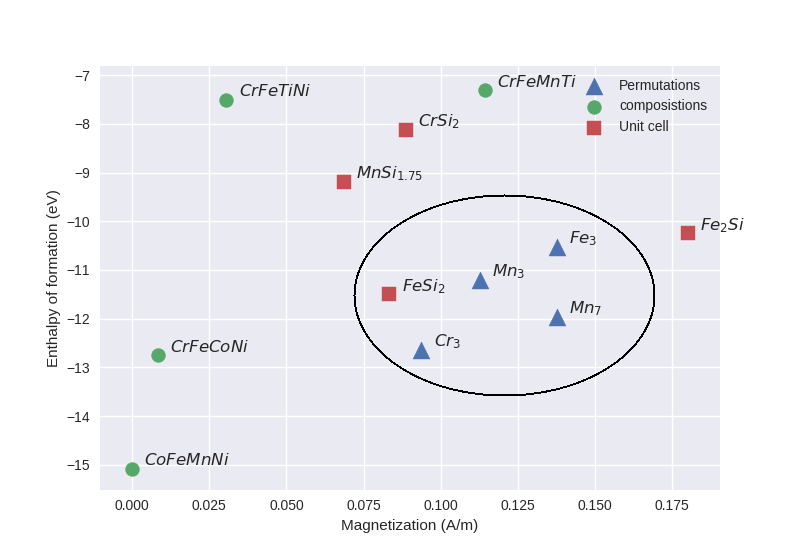
\includegraphics[width=\textwidth]{results/diagram.png}
\end{figure}